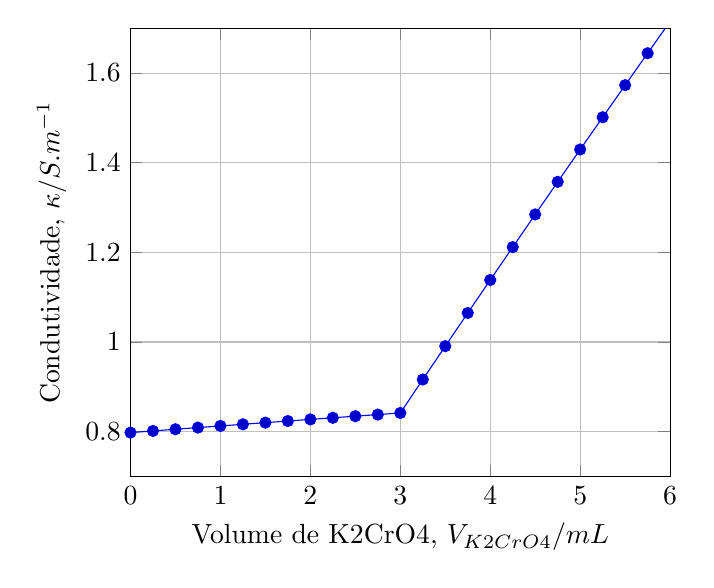
\begin{tikzpicture}
    \begin{axis}
        [
            grid = major,
            ylabel = {Condutividade, $\kappa/\unit{S.m^{-1}}$},
            xlabel = {Volume de \ce{K2CrO4}, $V_{\ce{K2CrO4}}/\unit{mL}$},
            domain = 0:6,
            xmin=0, xmax=6,
            ymin=0.7, ymax=1.7,
        ]
        \addplot
         {
             (
                 (7.35)*2*x*1 % K+
                 + (7.10)*6 % NO3-
                 + max((17)*(x - 3), 0) % CrO42-
                 + max((6.20)*(6 - 2*x*1), 0) % Ag+)
             )/(100 + x)
         };
 \end{axis}
 \end{tikzpicture}
 